% Created 2021-04-15 Thu 11:03
% Intended LaTeX compiler: pdflatex
\documentclass[presentation,bigger,aspectratio=169]{beamer}
\usepackage[utf8]{inputenc}
\usepackage[T1]{fontenc}
\usepackage{graphicx}
\usepackage{grffile}
\usepackage{longtable}
\usepackage{wrapfig}
\usepackage{rotating}
\usepackage[normalem]{ulem}
\usepackage{amsmath}
\usepackage{textcomp}
\usepackage{amssymb}
\usepackage{capt-of}
\usepackage{hyperref}
\usepackage{xcolor}
\usepackage[]{minted}
\usepackage{tcolorbox}
\usepackage{etoolbox}\tcbuselibrary{magazine}
\BeforeBeginEnvironment{minted}{\begin{tcolorbox}[title=Input,colback=blue!5,colframe=blue!25!black,size=fbox, enforce breakable, break at=6cm]}%
\AfterEndEnvironment{minted}{\end{tcolorbox}}%
\BeforeBeginEnvironment{verbatim}{\begin{tcolorbox}[colback=white,size=fbox,enhanced jigsaw, enforce breakable,break at=6cm]}%
\AfterEndEnvironment{verbatim}{\end{tcolorbox}}%
\usepackage{inconsolata}
\usepackage[ngerman, germanb]{babel}
\usepackage [autostyle, english = american]{csquotes} \MakeOuterQuote{"}
\usepackage[utf8]{inputenc}\usepackage{tabulary,booktabs}\AtBeginEnvironment{tabulary}{\scriptsize}
\usepackage[fixlanguage]{babelbib}\selectbiblanguage{german}
\usepackage{csquotes,xpatch}\usepackage[natbib=true,style=apa,url=true,doi=true,annotation=false,eprint=false,backend=biber]{biblatex}\urlstyle{sf}
\DeclareLanguageMapping{austrian}{austrian-apa}
\DeclareSourcemap{\maps[datatype=bibtex]{\map{\step[fieldset=annotation,null]}}}\renewcommand*{\bibfont}{\scriptsize}
\addbibresource{~/Dropbox/org/ref/ref.bib}
%Global Background must be put in preamble
\usebackgroundtemplate%
{%
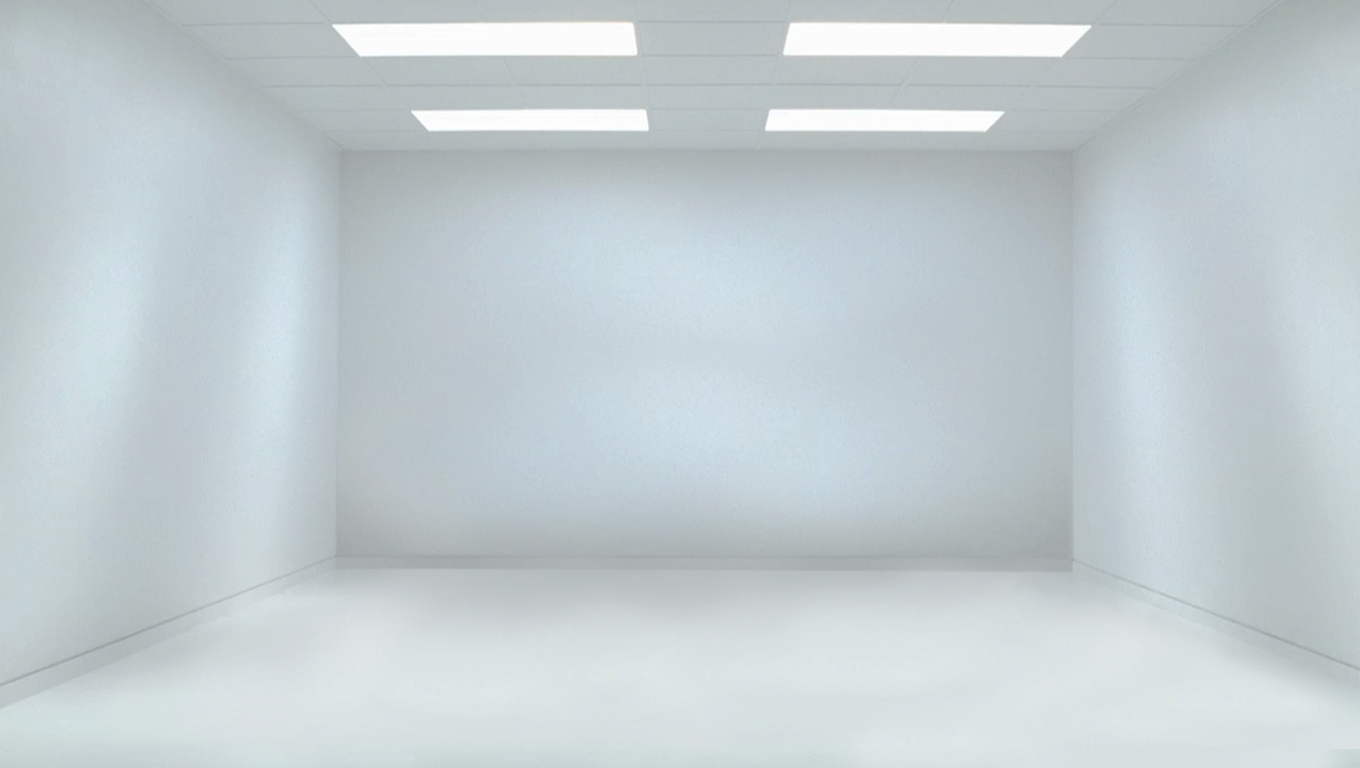
\includegraphics[width=1.175\paperwidth,height=1.05\paperheight]{./img/m1_praes_empty_10.jpg}%
}
\usetheme{default}
\author{user\thanks{user@mink}}
\date{15.4.2021}
\title{Interior Designer App: M1}
\subtitle{Problemanalyse}
\usetheme{Hannover}\usepackage{graphicx}\usepackage[overlay]{textpos}
\setbeamertemplate{bibliography item}{}
\setbeamertemplate{navigation symbols}{}
\definecolor{UBCblue}{HTML}{153a7a}\usecolortheme[named=UBCblue]{structure}
\usefonttheme{professionalfonts}
\setbeamerfont{note page}{family*=pplx,size=\footnotesize}
\definecolor{bgminted}{HTML}{eee9e9}
\definecolor{bluegray}{rgb}{0.54, 0.6, 0.8}
\definecolor{urlcolor}{HTML}{3399ff}
\definecolor{linkcolor}{HTML}{3399ff}
\definecolor{colorlinkscolor}{HTML}{3399ff}
\hypersetup{colorlinks=colorlinkscolor,linkcolor=linkcolor,urlcolor=urlcolor}
\setbeamertemplate{itemize items}[default]
\setbeamertemplate{enumerate items}[default]
\setbeamertemplate{items}[default]
\setbeamerfont*{title in sidebar}{shape=\scshape,size=\scriptsize}
\setbeamerfont*{author in sidebar}{family=\sfseries,size=\scriptsize}
\setbeamerfont*{section in sidebar}{family=\sfseries,size=\scriptsize}
\usetheme{Hannover}
\def\swidth{3.6cm}
\setbeamersize{sidebar width left=\swidth}
\setbeamertemplate{sidebar left}
{
{\usebeamerfont{title in sidebar}%
\vskip1.5em%
\usebeamercolor[fg]{title in sidebar}%
\insertshorttitle[width=\swidth,center,respectlinebreaks]\par%
\vskip1.25em%
}%
{%
\usebeamercolor[fg]{author in sidebar}%
\usebeamerfont{author in sidebar}%
\insertshortauthor[width=\swidth,center,respectlinebreaks]\par%
\vskip1.25em%
}%
\hbox to2cm{\hss\insertlogo\hss}
\vskip1.25em%
\hskip0.15cm\insertverticalnavigation{\swidth}%
\vfill
\hbox to2cm{\hskip0.25cm\usebeamerfont{subsection in
sidebar}\strut\usebeamercolor[fg]{subsection in
sidebar}\color{bluegray}\tiny\insertframenumber\hfill}%
\vskip6pt%
}%
\author[A.Oğuz, D.Pegler, S.Pum]{Asım Oğuz, Dominik Pegler, Sophia Pum}
\institute{Universität Wien, Fakultät für Informatik (SS2021)}
\hypersetup{
 pdfauthor={user},
 pdftitle={Interior Designer App: M1},
 pdfkeywords={},
 pdfsubject={},
 pdfcreator={Emacs 27.1 (Org mode 9.4.4)}, 
 pdflang={Germanb}}
\begin{document}

\maketitle

\section{Problembeschreibung}
\label{sec:orgbfbbe74}

\begin{frame}[label={sec:org3b7887a}]{\vspace{2.2cm}\begin{center}\MakeUppercase{\insertsection}\end{center}}
\end{frame}

\begin{frame}[label={sec:orga12a55c}]{Interior Designer App}
\begin{block}{Problemstellung}
\begin{enumerate}
\item Welche Gestaltungsmöglichkeiten bieten Räume?
\item Wie können Möbel sinnvoll angeordnet werden?
\item Wie können auch Laien schnell zu Raumlösungen kommen und diese
visualisieren?
\end{enumerate}
\end{block}
\end{frame}
\begin{frame}[label={sec:org6458e70}]{Interior Designer App}
\begin{block}{Lösungsansatz: Mobile App}
\begin{itemize}
\item User fotografiert Raum
\item User wählt Möbelstück
\item App vermisst Raum, Möbelstück
\item User/App platziert Möbelstück im Raum
\end{itemize}
\vspace{0.8em}\hspace{2em}{\bfseries {\Longrightarrow} {\text{Augmented-Reality-Lösung (AR)}}}
\end{block}
\end{frame}

\begin{frame}[label={sec:orgdae2f0d}]{Interior Designer App}
\begin{block}{Zusätzliches Feature: "Open Objects Sharing" ("OOS")}
\begin{itemize}
\item 3D-Objekte können einfach erstellt und an andere Personen geschickt werden
\item Integration in Second-Hand-Apps wie Shpock oder Willhaben
\end{itemize}
\end{block}
\end{frame}

\section{Literaturrecherche}
\label{sec:orgcf1d66d}
\begin{frame}[label={sec:org4248cea}]{\vspace{2.2cm}\begin{center}\MakeUppercase{\insertsection}\end{center}}
\end{frame}

\begin{frame}[label={sec:org565a545}]{Literatur}
\begin{block}{Schwerpunkt Algorithmen und Augmented Reality}
\begin{itemize}
\item Algorithmus, der Räume selbstständig befüllt

\parencite{kanAutomatedInteriorDesign2017}
\item Augmented-Reality-Framework ArToolKit

\parencite{sanduAugmentedRealityUses2018}
\item Erstellung AR-Interior-App mit Google Cardboard SDK

\parencite{moaresInterARInterior2020}
\end{itemize}
\end{block}
\end{frame}

\begin{frame}[label={sec:org27ef1d2}]{Literatur}
\begin{block}{Takeaways}
\begin{itemize}
\item auf Bestehendem aufbauen ("Einrichtungs"-Algorithmen \&
Augmented-Reality-Lösungen gibt es bereits)
\item Wahl des AR-Frameworks miteinscheidend über den Funktionsumfang
\item Auch leere Räume ermöglichen
\item Durch Algorithmus eingerichtete Räume werden als gut bewertet
\end{itemize}
\end{block}
\end{frame}

\section{Konkurrenzanalyse}
\label{sec:orgcce30e9}
\begin{frame}[label={sec:org6bb5f8c}]{\vspace{2.2cm}\begin{center}\MakeUppercase{\insertsection}\end{center}}
\end{frame}

\begin{frame}[label={sec:org0d4c6ec}]{Konkurrenzanalyse I}
\begin{block}{Houzz}
\vskip 0.7em 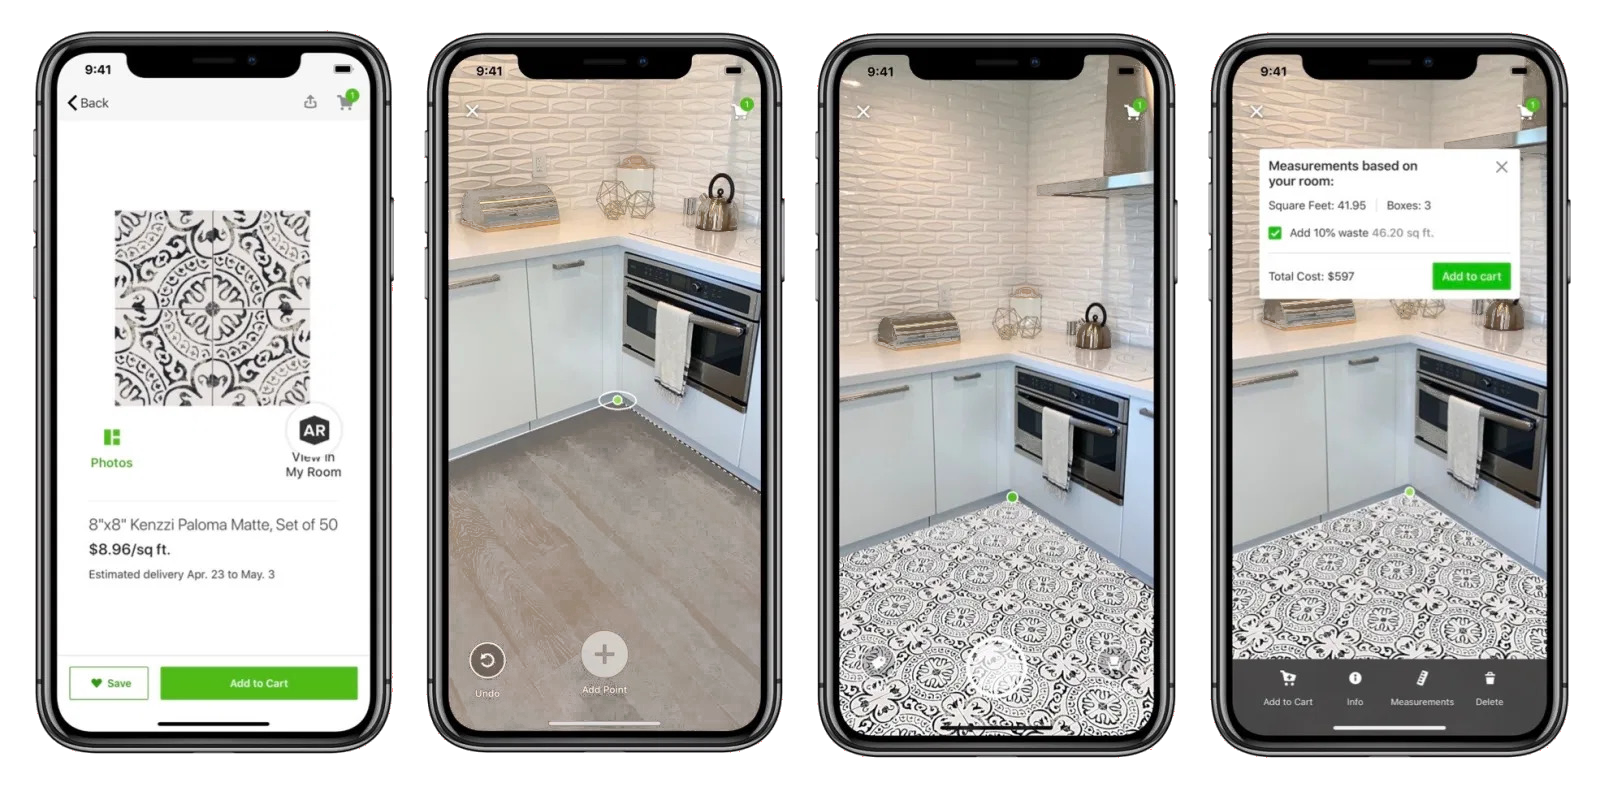
\includegraphics[width=25em]{./img/m1_praes_houzz.png}
\end{block}
\end{frame}

\begin{frame}[label={sec:orgf559e44}]{Konkurrenzanalyse I}
\begin{block}{Houzz}
\begin{itemize}
\item Bilder von verschiedenen Einrichtungen zu Inspiration
\item Persönliche Entwürfe mithilfe AR-Technologie
\item Nachteil: Spezialisierung auf Häuser/ große Räume.
\end{itemize}
\end{block}
\end{frame}
\begin{frame}[label={sec:org8172078}]{Konkurrenzanalyse II}
\begin{block}{Ikea Place}
\vskip 0.7em 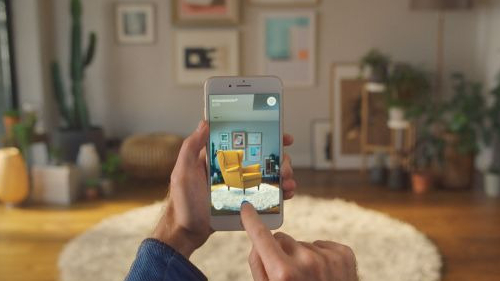
\includegraphics[width=25em]{./img/m1_praes_ikea.jpg}
\end{block}
\end{frame}
\begin{frame}[label={sec:org7c4b393}]{Konkurrenzanalyse II}
\begin{block}{Ikea Place}
\begin{itemize}
\item Eigene Räume mit Ikea-Produkte digital einrichten
\item Verschiedene Möbel ausprobieren und direkt bestellen
\item Nachteil: Auf Ikea Möbel beschränkt
\end{itemize}
\end{block}
\end{frame}
\begin{frame}[label={sec:org63a1db3}]{Konkurrenzanalyse III}
\begin{block}{Homestyler}
\vskip 0.7em 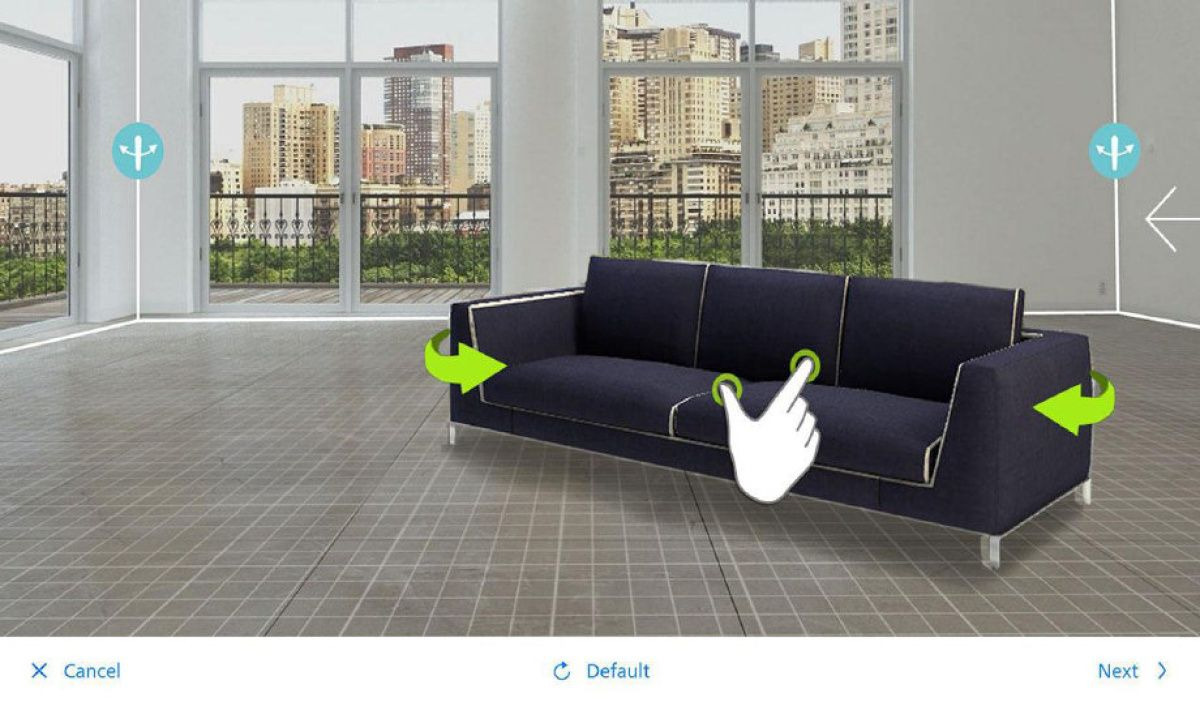
\includegraphics[width=25em]{./img/m1_praes_homestyler.jpg}
\end{block}
\end{frame}
\begin{frame}[label={sec:orgee51e5f}]{Konkurrenzanalyse III}
\begin{block}{Homestyler}
\begin{itemize}
\item Eigene Räume umgestalten und bearbeiten
\item Verschiedene Farben, Materialien und Möbel
\item Viele Gestaltungsmöglichkeiten in verschiedenen Stilen
\end{itemize}
\end{block}
\end{frame}
\section{Nutzeranalyse}
\label{sec:orgcd3d92f}
\begin{frame}[label={sec:orgd04fef0}]{\vspace{2.2cm}\begin{center}\MakeUppercase{\insertsection}\end{center}}
\end{frame}

\begin{frame}[label={sec:org7a903e8}]{Nutzeranalyse I}
\begin{block}{Aufgaben der Nutzer}
\begin{itemize}
\item Schnelles Skizzieren von Innenarchitekturen
\item Schnelles Visualisieren
\item Anderen Personen vorführen
\end{itemize}
\end{block}
\end{frame}
\begin{frame}[label={sec:org7934111}]{Nutzeranalyse II}
\begin{block}{Ziele der Nutzer}
\begin{itemize}
\item Zeit- und Kostenersparnis (keine Beratung nötig)
\item Konkretere Vorstellungen zu entwickeln
\item Bessere und nachhaltigere Entscheidungen treffen
\end{itemize}
\end{block}
\end{frame}

\begin{frame}[label={sec:org455f896}]{Nutzeranalyse III}
\begin{block}{Potenzielle Probleme mit dem System}
\begin{itemize}
\item User fühlen sich von App nicht angesprochen
\item Kein Zusatznutzen zu bereits vorhandenen Tools
\item Funktionalitäten zu eingeschränkt (nur bestimmte Möbel/Objekte,
Limit bei Anzahl)
\item Aufbau und Logik des Programms zu kompliziert
\item Zu lange Ladezeiten (bei mobilen Apps besonders wichtig!)
\item Freezing oder Absturz der App
\item Läuft nicht auf allen Smartphones
\end{itemize}
\end{block}
\end{frame}

\section{Personas}
\label{sec:orgb47b238}
\begin{frame}[label={sec:org2748114}]{\vspace{2.2cm}\begin{center}\MakeUppercase{\insertsection}\end{center}}
\begin{center}
\vskip -12.5em 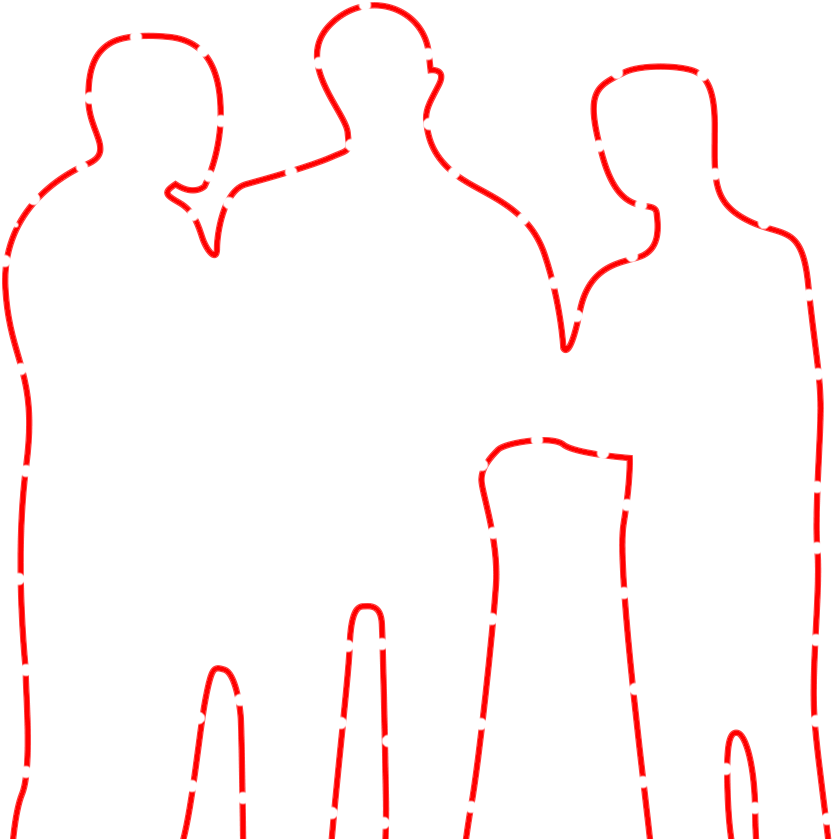
\includegraphics[height=140px]{./img/m1_praes_ol_persona3.png}
\end{center}
\end{frame}
\begin{frame}[label={sec:orgab336b1}]{Personas I}
\begin{block}{Primäre Persona 1: Tobias Ebner}
\begin{center}

\includegraphics[width=90px]{./img/m1_persona_1_idealist.png}
\end{center}
\begin{itemize}
\item Typ: Idealist
\item Alter: 25
\item Beruf: Grafikdesigner
\end{itemize}
\end{block}
\end{frame}
\begin{frame}[label={sec:org9131927}]{Personas II}
\begin{block}{Primäre Persona 2: Carina Winkler}
\begin{center}
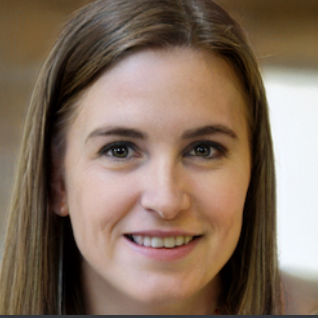
\includegraphics[width=90px]{./img/m1_persona_2_rational.png}
\end{center}
\begin{itemize}
\item Typ: Rational
\item Alter: 32
\item Beruf: Ärztin
\end{itemize}
\end{block}
\end{frame}
\begin{frame}[label={sec:org2ccdedb}]{Personas III}
\begin{block}{Sekundäre Persona: Felix Schuster}
\begin{center}
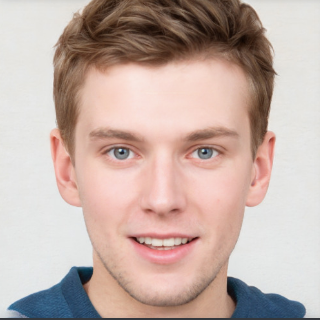
\includegraphics[width=90px]{./img/m1_persona_3_rational.png}
\end{center}
\begin{itemize}
\item Typ: Minimalist
\item Alter: 20
\item Beruf: Student
\end{itemize}
\end{block}
\end{frame}
\begin{frame}[label={sec:orge81bb62}]{Personas IV}
\begin{block}{Negative Persona: Sabine Gruber}
\begin{center}
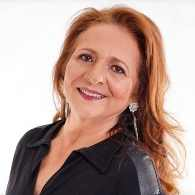
\includegraphics[width=90px]{./img/m1_persona_4_guardian.jpg}
\end{center}
\begin{itemize}
\item Typ: Guardian
\item Alter: 64
\item Beruf: Verkäuferin
\end{itemize}
\end{block}
\end{frame}
\section{Aufgabenanalyse}
\label{sec:org829daff}
\begin{frame}[label={sec:org0ccb53f}]{\vspace{2.2cm}\begin{center}\MakeUppercase{\insertsection}\end{center}}
\end{frame}
\begin{frame}[label={sec:org511d018}]{Aufgabenanalyse}
\begin{center}
\begin{tabular}{lcc}
\toprule
\(\downarrow\) Task / User \(\to\) & Carina Winkler & Tobias Ebner\\
\midrule
App downloaden & + & +\\
Raum fotografieren & + & +\\
Möbel scannen & \textasciitilde{} & \textasciitilde{}\\
Vorhandene Möbel auswählen & + & +\\
Raum gestalten & \textasciitilde{} & \textasciitilde{}\\
Design abspeichern & + & +\\
\bottomrule
\end{tabular}
\end{center}
\end{frame}

\section{Projektmanagement}
\label{sec:org50005ca}
\begin{frame}[label={sec:orga112e22}]{\vspace{2.2cm}\begin{center}\MakeUppercase{\insertsection}\end{center}}
\end{frame}

\begin{frame}[label={sec:orgef9b341}]{Projektmanagement I}
\begin{block}{Abstimmung und Planung}
\begin{itemize}
\item Simple Github-Page mit
\begin{itemize}
\item TODOs
\item Terminen und Deadlines
\item Zuordnung der Aufgaben
\item Notizen
\item Updates zum Fortschritt
\end{itemize}
\end{itemize}
\end{block}
\end{frame}


\begin{frame}[label={sec:org4cee048}]{Projektmanagement II}
\begin{block}{Ziele des Projekts}
\begin{itemize}
\item Prototyp einer App entwickeln, die so simpel wie möglich ist
\item Zumindest Teile des Projekts später in Realität umsetzen
\item Neue Technologien kennenlernen
\end{itemize}
\end{block}
\end{frame}
\begin{frame}[label={sec:orgfa96209}]{Projektmanagement III}
\begin{block}{Nicht-Ziele des Projekts}
\begin{itemize}
\item Bestehendes wiederholen
\item Nice-To-Have-Features ohne relevanten Zusatznutzen implementieren (z.B. weil
die Technik dahinter spannend ist) \(\to\) alles weglassen, das nicht mit
den Nutzerzielen zu tun hat
\end{itemize}
\end{block}
\end{frame}

\section*{Literatur}
\label{sec:org29cfa70}
\begin{frame}[allowframebreaks]{Literatur}
\printbibliography[heading=none]
\end{frame}
\appendix
\end{document}
